\section{Results}
% NOTE:
% You are expected to refer to all the floats (figures, tables, etc.)
% in the results section.

% shows how to create a table and how to refer to it
Table~\ref{t:time} shows the average number of operations and elapsed
times (nanoseconds) for increasing input sizes.

\begin{table}[H]	% uses float package to control placement
	\centering	% centers the table
	\caption{
		The number of operations and the elapsed time (nanoseconds)
		as a function of the input size.
	}	% provides a concise description of the table contents

	\begin{tabular}{r r r}
		% table header
		size & operations & elapsed time \\
		% inserts horizontal line
		\hline
		% separates column entries with the ampersand &
		10& 35& 1997800316711600 \\
		12& 44& 1997945809898000 \\
		20& 105& 1998047688985600 \\
		22& 121& 1997984288534200 \\
		24& 149& 1998012627163400 \\
		30& 227& 1998172719441100 \\
		42& 436& 1998192378544300 \\
		50& 616& 1998242758918400
	\end{tabular}

	% defines a label to refer to it
	\label{t:time}
\end{table}


A graph of the average number of operations and the runtime is given in
figure~\ref{fig:best}.

\begin{figure}[H]
	%centers the figure
	\centering
	% my LaTeX installation expects Encapsulated PostScript EPS graphs
	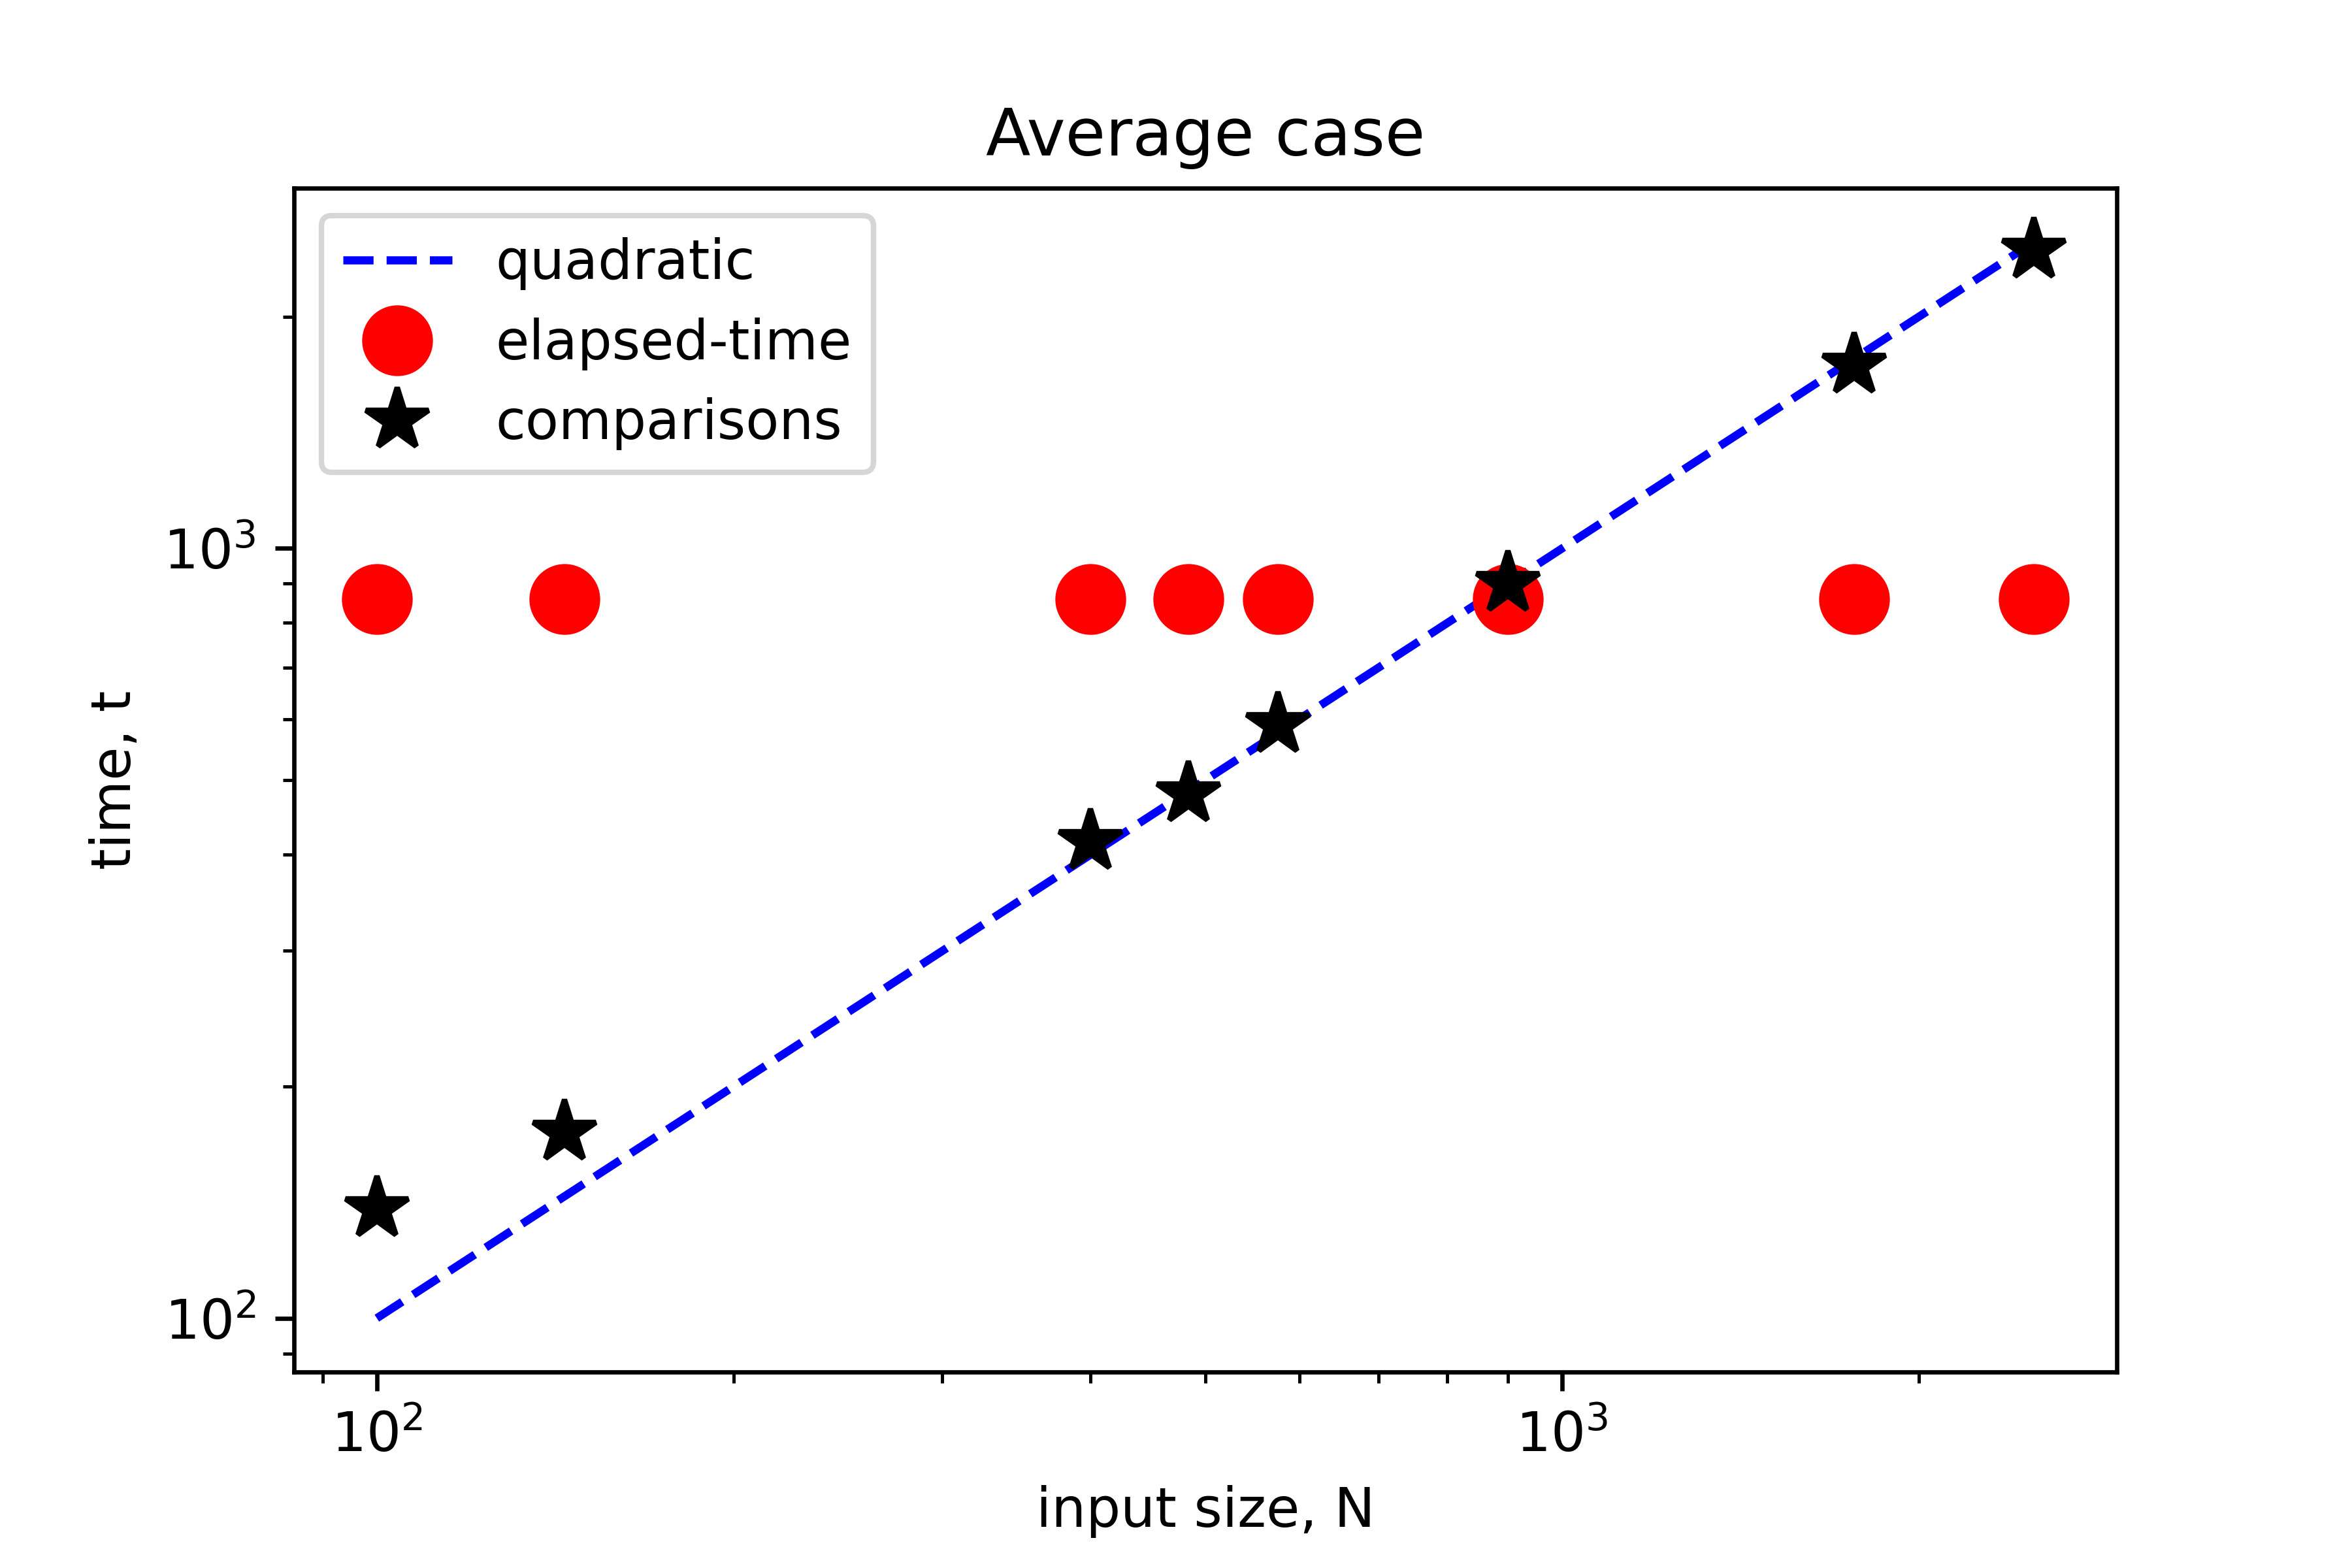
\includegraphics[keepaspectratio]{average.jpeg}
    \caption{
		The average number of operations and runtime as a function of the input size $N$.
	} 
    
	% defines a label to refer to it
	\label{fig:best}
\end{figure}